%!TEX TS-program = xetex
\documentclass{TDP005mall}
\usepackage[utf8]{inputenc}
\usepackage[swedish]{babel}
\usepackage[export]{adjustbox}
\usepackage{tabularx}
\usepackage{caption}
\usepackage{csquotes}

\renewcommand*{\contentsname}{Innehållsförteckning}

\newcommand{\version}{Version 1.2}
\author{Daniel Huber, \url{danhu849@student.liu.se}\\
  Viktor Rösler, \url{vikro653@student.liu.se}}
\title{Designspecifikation}
\date{2020-11-27}
\rhead{Daniel Huber\\
Viktor Rösler}

% For aligning captions to the left.
\captionsetup{justification=raggedright,singlelinecheck=false} 

\begin{document}
\projectpage
\tableofcontents
\newpage
\section{Revisionshistorik}
\begin{table}[!h]
\begin{tabularx}{\linewidth}{|l|X|l|}
\hline
Ver. & Revisionsbeskrivning & Datum \\\hline
1.2 & Detaljbeskrivning och externa filformat & 201127 \\\hline
1.1 & Klassdiagram och designdiskussion & 201125 \\\hline
1.0 & Designspecifikation 1:a utkast & 201125 \\\hline
\end{tabularx}
\end{table}


% TODO
% Läs CC, Primer och Design Patterns
% Notera sidor
% Skriv in Källor i dokumentet
% Skriv detaljbeskrivningarna.
% Kötta fram en diskussion.
% KLART

\section{Klassdiagram}
% Viktigaste innehållet i designspecen är ett klassdiagram som visar den objektorienterade designen av spelet.
% Klassdiagram enligt UML som beskriver hela ert system. Diagrammet skall vara kommunikativt och beskriva hela systemets inre uppbyggnad och funktion. Klassdiagrammet ska innehålla alla relationer som finns mellan era klasser. För associationer ska det framgå vilken riktning samt multiplicitet relationerna har. 

\begin{figure}[h!]
  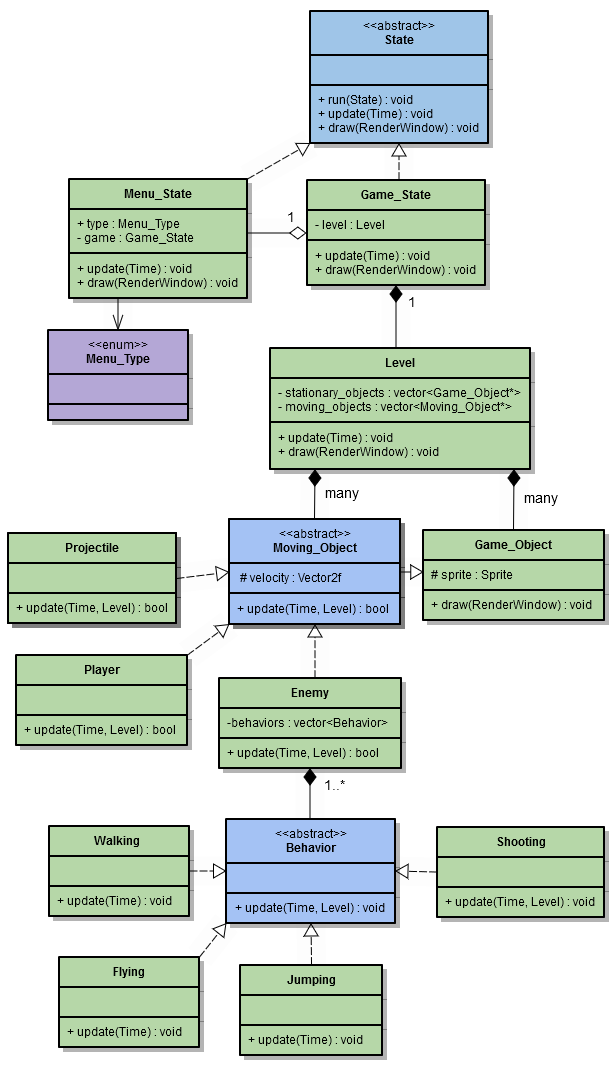
\includegraphics[height=16cm]{UML1.2.png}
  \caption{Klassdiagram\label{fig:1}}
\end{figure}

\section{Designdiskussion}
% En kort diskussion (1/2-1 sida) där ni motiverar er design och tar upp fördelar och nackdelar med den. Diskutera gärna också om det är något ni tycker är dåligt med den, och beskriv alternativa, bättre lösningar. 

% CC sida 104.

Klassen \verb|State| och dess underklasser \verb|Game_state| och \verb|Menu_State| representerar tillståndet spelet befinner sig i. Endast ett state är aktivt åt gången; \verb|Game_State| om spelet är igång, eller \verb|Menu_State| om spelaren befinner sig i en meny. Ett \verb|Menu_State| innehåller ett \verb|Game_State| som ritas ut bakom menyn. Anledningen till det är att vi vill få till en snygg övergång mellan \verb|Menu_State| och \verb|Game_State|. När spelet övergår från \verb|Menu_State| till \verb|Game_State| försvinner menyn från skärmen, och nivån som ritades ut bakom menyn blir spelbar. En nackdel med att ha ett \verb|Game_State| i \verb|Menu_State| är att spelet kan behöva att läsa in fler nivåer än de som spelas. T.ex. när spelaren bläddrar i nivåmenyn ska den nivå som är markerad visas i bakgrunden, men det är inte säkert att spelaren väljer att spela den nivån. Det vore lämpligt om vi endast behöver läsa in varje nivå högst en gång, oavsett hur många gånger den ska användas. Vi har gjort avvägningen att läsa in nivåer och behålla dem i minnet är mer effektivt än att behöva läsa in respektive nivå varje gång den väljs av användaren. Det skulle kunna genomföras med en singleton-klass som endast har ansvaret att läsa in och komma ihåg nivåer.

\verb|Menu_State| kan representera olika sorters menyer, t.ex. en startmeny, en pausmeny eller en meny för inställningar. Vilken sorts meny ett \verb|Menu_State| objekt representerar bestäms när objektet skapas. För att dölja implementationen av \verb|Menu_State| från andra klasser, och få till bra inkapsling, anropas konstruktorn till \verb|Game_Menu| med en uppräkningstyp (enumeration) som argument. Uppräkningstypen bestämmer vilken typ av meny som ska skapas.

Klassen \verb|Level| representerar en nivå i spelet. Klassen innehåller två vektorer med de objekt nivån består av, objekt som ändrar nivåkoordinater, \verb|Moving_Object| och objekt som har statiska nivåkoordinater, \verb|Game_Object|. Uppdelningen finns för att endast behöva anropa en update-funktion på de objekt som behöver uppdateras under spelets gång och för att kunna uppdatera objekt av typen \verb|Moving_Object| ovanför spelfönstrets vy.

Varje \verb|Game_Object| ritas ut genom att \verb|draw| funktionen i \verb|RenderWindow| klassen anropas med \verb|Game_Object| objektets \verb|Sprite| medlem som argument. Det fungerar för att \verb|Game_Object| ärver från sfml-klassen \verb|Drawable|. Det gör att alla underklasser till \verb|Game_Object| också kan ritas ut. En nackdel är att \verb|Game_Objekt| blir större än nödvändigt, i form av den extra funktionalitet som finns i \verb|Sprite| klassen. T.ex. har \verb|Sprite| klassen en funktion för att flytta på sig, men ett objekt av typen \verb|Game_Object| behöver inte kunna göra det.

Funktionen \verb|update| anropas i gameloopen i \verb|Game_State| som i sin tur anropar \verb|update| i \verb|Level| ner till \verb|update|-funktionerna i varje \verb|Behavior|. Varje objekt ska uppdatera sig själv och skicka anropet vidare nedåt. De \verb|Game_Object| varje klass behöver ska känna till så lite som möjligt om de andra klasserna i kedjan, men \verb|Level| behöver skicka sig själv vidare så att objekt av typen \verb|Moving_Object| kan veta om de kolliderar med andra objekt i nivån eller inte. \verb|update| funktionen i \verb|Moving_Object| och dess underklasser returnerar en bool för att \verb|Level| ska kunna avgöra om objektet ska tas bort eller inte.

Ett objekt av typen \verb|Enemy| består av ett antal beteenden. Varje beteende är ett objekt av någon undertyp till den abstrakta klassen \verb|Behavior|. När funktionen \verb|update()| anropas på ett \verb|Enemy|-objekt uppdateras objektet enligt de beteenden denna fienden har. Poängen med att bryta ut fiendernas beteenden från \verb|Enemy|-klassen är att det ska vara lätt att utöka spelet med fler fiendetyper. Vi har bossfiender som ett bör-krav till projektet. Det kravet ska kunna genomföras genom att vi återanvänder, och skapar nya, beteenden till den redan existerande \verb|Enemy|-klassen utan att behöva skapa en ny klass för bossar.  

\section{Detaljbeskrivning av klassen Player}
Klassen \verb|Player| representerar en figur i en nivå som en spelare kan styra. Det finns ett \verb|Player| objekt per spelare i varje nivå, och varje \verb|Player| objekt skapas och förtstörs tillsammans med nivån den är en del av. \verb|Player| ärver från den abstrakta klassen \verb|Movable_Objekt| som representerar alla typer av objekt i en nivå som kan flytta på sig. \verb|Movable_Objekt| ärver i sin tur från klassen \verb|Game_Objekt|, vilket är basklassen för alla typer av objekt i en nivå som har kollisionshantering.    

\subsection{Medlemmar i klassen Player}
\subsubsection{Konstruktor:}
\begin{itemize}
  \item  \verb|Player(Sprite sprite)| - Skapar ett spelarobjekt på den position som \verb|sprite| har, med den grafik som \verb|sprite| använder. Använder konstruktorn i \verb|Moving_Objekt|, och konstruktorn i \verb|Moving_Object| använder kontruktorn i \verb|Game_Object|.
\end{itemize}

\subsubsection{Funktioner:}
\begin{itemize}
  \item (public) \verb|bool update(Time time, Level level)| - Uppdaterar spelarobjektet baserat på spelaren knapptryckningar. Parametern \verb|level| används för att lägga till projectiler i nivån när spelaren skjuter. Funktionen anropar \verb|update| funktionen i \verb|Moving_Object|.
\end{itemize}

\subsubsection{Variabler:}
\begin{itemize}
  \item (private) \verb|int health| - Antal liv spelaren har, [0, 3].
\end{itemize}

\subsection{Arv från klassen Moving\_Object}
\subsubsection{Funktioner:}
\begin{itemize}
  \item (public) \verb|bool update(Time time, Level level)| - Uppdaterar objektets position. Returvärdet anger om objektet vill bli borttaget eller ej. 
\end{itemize}

\subsubsection{Variabler:}
\begin{itemize}
  \item (protected) \verb|Vector2f velocity| - Anger hur snabbt, och i vilken riktning, ett objekt ska flytta på sig. 
 % \item (protected) \verb|int anim_count| - Antal olika bilder i objektets animation. 
 % \item (protected) \verb|Time anim_speed| - Hur länge varje bild i objektets animation ska visas. 
\end{itemize}

\subsection{Arv från klassen Game\_Object}
\subsubsection{Funktioner:}
\begin{itemize}
  \item (public) \verb|void draw(RenderWindow window)| - Ritar ut ett objekt på skärmen.
\end{itemize}

\subsubsection{Variabler:}
\begin{itemize}
  \item (protected) \verb|Sprite sprite| - Innehåller objektets position och grafik. 
\end{itemize}

\section{Detaljbeskrivning av klassen Level}
Klassen \verb|Level| representerar en nivå i spelet som kan spelas. Ett \verb|Level| objekt innehåller pekare till alla \verb|Game_Objekt| och \verb|Moving_Objekt| som nivån består av, och tillhandahåller två funktioner som objekten i en nivå anropar. \verb|add_object| funktionen låter ett skjutande objekt lägga till projektilen i nivån, och \verb|check_collisions| funktionen kollar om ett objekt kolliderar med något annat objekt i nivån.

\subsection{Medlemmar i klassen Level}
\subsubsection{Konstruktor:}
\begin{itemize}
  \item  \verb|Level(String file_name, bool multiplayer)| - Anropar \verb|load_level| med \verb|file_name| som argument för att läsa in en nivå från en .csv fil. \verb|multiplayer| parametern anger om nivån ska spelas av två spelare eller ej.
  
\end{itemize}

\subsubsection{Funktioner:}
\begin{itemize}
  \item (public) \verb|bool update(Time time)| - Anropar \verb|update| på alla objekt i \verb|moving_objects|, med både \verb|time| och sig själv´som argument.
  \item (protected) \verb|vector<Game_Object*> check_collisions(Game_Object object)| - Retunerar en vektor med pekare till alla objekt i nivån som kolliderar med \verb|object|.
  \item (protected) \verb|void add_object(Moving_Object* object)| Lägger till objektet \verb|object| i \verb|moving_objects| vektorn. Används av \verb|Enemy| och \verb|Player| klasserna för att lägga till projektiler i nivå.
  \item (private) \verb|void load_level(String file_name)| - Läser in en nivå från en .csv fil.
  
\end{itemize}

\subsubsection{Variabler:}
\begin{itemize}
  \item (private) \verb|vector<Game_Object*> stationary_objects | - Vektor med alla stillastående objekt som nivån består av.
    \item (private) \verb|vector<Moving_Object*> moving_objects | - Vektor med alla rörliga objekt som nivån består av. De två första objekten i vektorn ska vara \verb|Player objekt. Det gör att \verb|Level| kan avgöra vilka objekt som är av typen \verb|Player| utan att skapa ett direkt beroende mellan klasserna. Det ena \verb|Player| objektet ska endast ritas ut och uppdateras om flerspelarläget är på. 
    
    \item (private) \verb|bool multiplayer| - Avgör om spelare två ska ritas ut och uppdateras.
\end{itemize}

\section{Externa Filformat}
% Beskriv de externa filformat ni använt i ert spel, till exempel för highscore-listor eller banbeskrivningar. Detta är kanske inte relevant för alla, då man kan lösa uppgiften utan användning av externa format.
Nivåerna läses in i spelet från .csv filer där varje nivå utgör en .csv fil. I .csv filen finns data gällande hur många tiles som nivåns bredd respektive höjd utgör. Filen innehåller också information om alla sprites koordinater för dess startposition. 


\end{document}

%%% Local Variables: 
%%% coding: utf-8
%%% mode: latex
%%% TeX-engine: xetex
%%% TeX-master: t
%%% End: 



